\section{Result}
This section covers the results of this project. It will explain, how the final workflow works and what kind of product were produced during the time of this bachelor thesis.

\subsection{Discussion}
\label{sub:Discussion}

\subsection{Workflow}
During the time of this project, we tried out different algorithms and processes (Section~\ref{sub:Discussion}), to create a workflow, which solves the stated task (Section~\ref{sub:ProblemDescription}).

\begin{figure}[H]
	\centering
	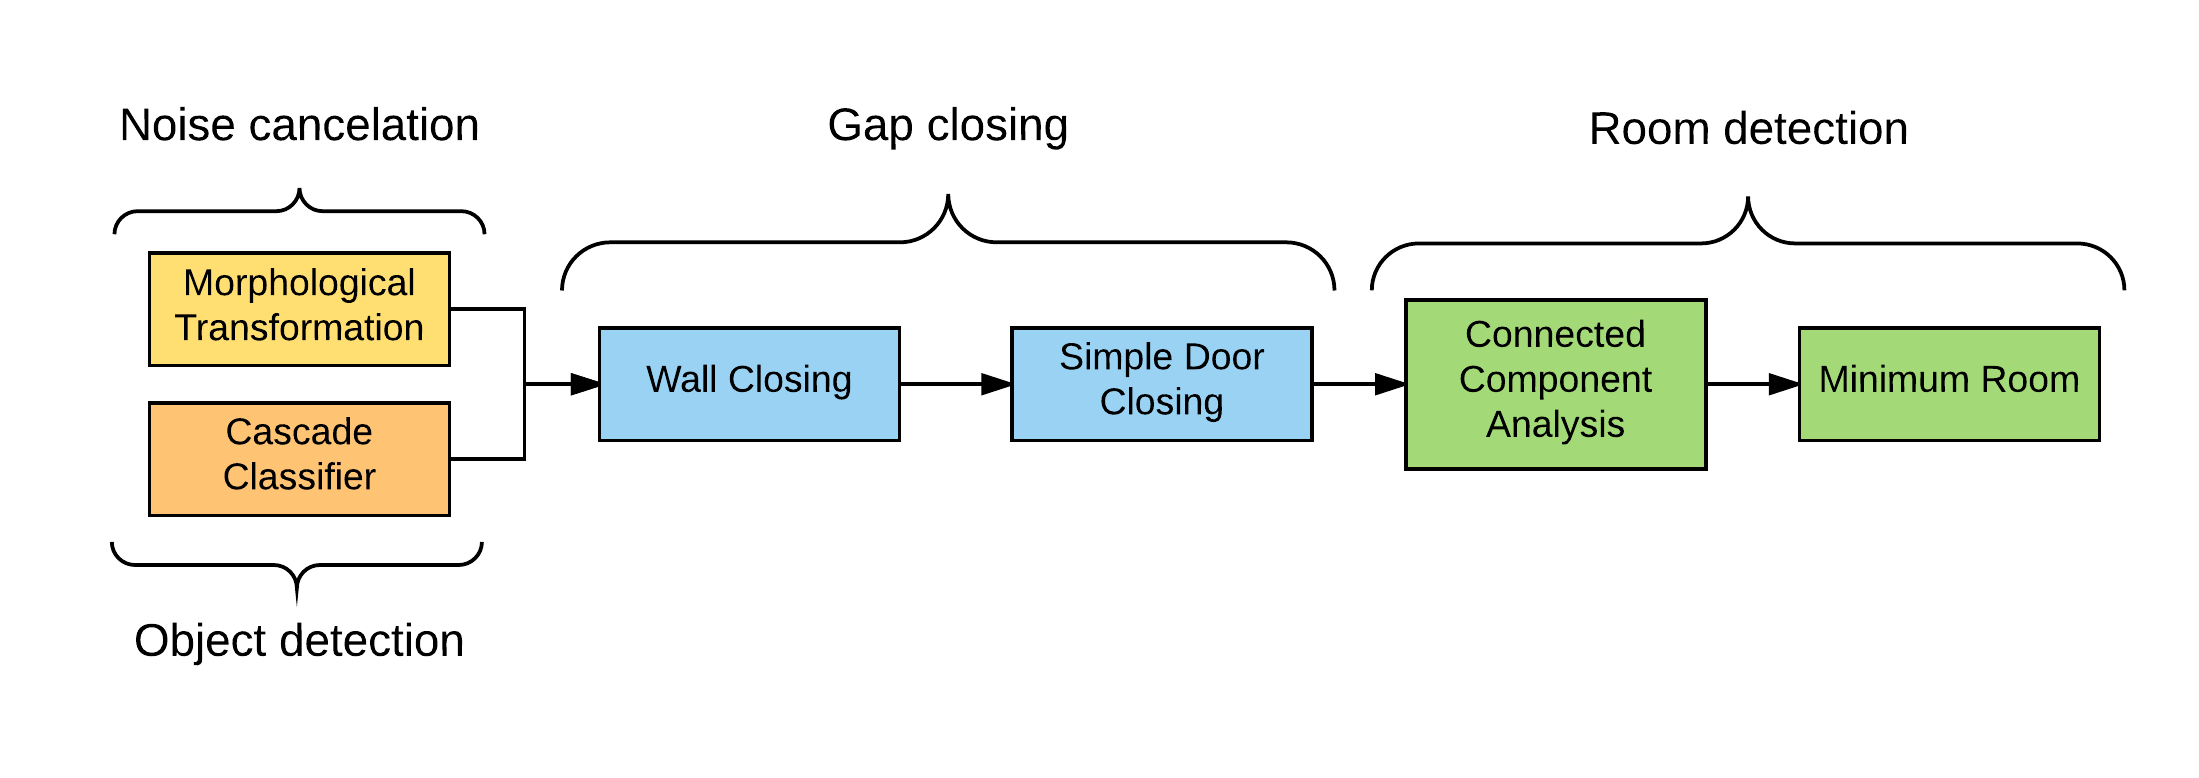
\includegraphics[width=1.0\textwidth]{FinalWorkflow}
	\caption{Final workflow flowchart.}
	\label{fig:FinalWorkflow}
\end{figure}

The workflow is visualised in figure~\ref{fig:FinalWorkflow} is the same workflow as the workflow three, described in section~\ref{sub:workflow3}.

It starts with the object detection (Section~\ref{sub:ObjectDetection}), which detects all doors on a floor plan. This information is saved into the meta image format (Section~\ref{sub:MetaFormat}) for further processing. Then the noise cancelation (Section~\ref{sub:NoiseRemoval}) removes noise like furniture, markings and other elements on the plan, to create a skeleton of the building walls.

Due the fact, that the noise cancelation removes also the windows of the building, the wall closing algorithm (Section~\ref{sub:WallClosing}) finds the outer contour and closes the gaps. Together with the information gathered in the objection detection step, the simple door closing algorithm (Section~\ref{sub:SimpleDoorClosing}) closes the gaps between the walls, where the doors should be.

After the cleanup and reconstruction process, the room detection is processed (Section~\ref{sub:RoomDetection}). As final step, the minimum room detection (Section~\ref{sub:MinimumRoom}) filters out rooms, which are too small, in relation to the average room size.


\subsection{Prototype}

\subsection{Limitations and restrictions}